%# -*- coding: utf-8-unix -*-
%%==================================================
%% chapter01.tex for SJTU Master Thesis
%%==================================================

%\bibliographystyle{sjtu2}%[此处用于每章都生产参考文献]
\chapter{系统设计}
\label{chap:systemdesign}
DOBBS是为了适应大规模IaaS云的底层存储,利用对象存储对非结构化数据VMDI进行大量优化,并且在WHOBBS的基础上解决了其性能缺陷。本章我将介绍DOBBS的
系统架构设计以及各模块设计。

\section{设计目标}
对于混合存储的研究,我们已经有了WHOBBS\cite{lingxuan2015whobbs}和MOBBS\cite{ma2014mobbs}两个系统。而我们的DOBBS是在WHOBBS的基础上进行的改进。
WHOBBS通过动态监测虚拟机VMDI对象的访问数据流信息,然后客户端收集到对象的数据数据数据流信息之后定时发送给独立的监控器服务器。监控器服务器中的分析器模块则
负责收集对象信息,然后根据特定的对象热度计算算法,让较“热”的对象放置于SSD而较“冷”的对象放置于HDD,并且通过动态监测实现SSD和HDD上对象的动态迁移。因此,
WHOBBS系统主要包含三个部分,客户端、监控器和存储集群,它们通过网络连接。其中整个系统的核心就是监控器,监控器保存了每个对象的数据流信息,而且还一直在计算
对象的热度,发送迁移指令。在WHOBBS的实现上,作者让系统仅存在一个监控器服务器,它负责收集所有接入客户端的信息并产生决策。

考虑WHOBBS的系统架构,我们可以看到监控器节点是整个系统的大脑和决策者,它不仅保存数据还进行大量的计算。在\citen{barroso2013datacenter}一书中,作者提到
基于Web的计算和面向服务的计算必须要保证高可靠性,用户才会信任它。但是WHOBBS的单一监控器架构导致了这个监控器成为系统的唯一关键节点,这就意味着一旦这个节点所在
的物理机宕机、网络不能访问或者软件出现异常,对整个系统都会造成极大的影响。可以试想,如果监控器宕机,那么客户端则不能讲记录的对象数据流信息发送给监控器,并且
底层存储集群内的对象不能被迁移,整个系统则处于一个没有被优化的状态。

对于WHOBBS的架构中监控器可能存在的唯一关键节点的问题,本实验室的RHOBBS\cite{zhenwang2016rhobbs}就是准备用于解决这个问题。它采用了多复制的策略,架构
不再采用单一监控器的模式,而是采取了多个类监控器节点,叫做Shuffler。它们保存客户端发送过来的对象数据流信息的相同副本,并且通过Raft一致性协议保证了Shuffler间
副本的一致性。并且它基于Raft算法,实现了Shuffler的错误恢复,一旦出现宕机的情况可以保证可以通过其他Shuffler来进行数据的热度计算等工作。

但是可以想到,由于WHOBBS的监控器保存的数据仅仅是对象的数据流信息而并不是实际的对象数据,那么如果监控器宕机,虚拟机仍然可以和底层存储进行交互,只是SSD不会被充分利用,
实质上虚拟机的运行不会受到太大影响。因此,如果从保证监控器的高可用性的角度出发去优化没有特别紧迫的重要性。我们回到WHOBBS的系统设计,监控器只有一个,它要接受所有接入客户端
的数据流信息,然后将信息储存下来,再调用分析线程逐渐计算所有对象的热度。考虑监控器的实现,它将数据流信息放置于内存中,并且分析线程则不断地对所有内存内的数据排序、遍历和运行
热度计算算法。虽然热度计算算法的算法复杂度并不高,但是对所有数据排序是会占有较多的CPU时间。如果当系统逐渐庞大,有越来越多的客户端接入系统,同一个监控器节点要同时接受所有
客户端的网络连接。现在WHOBBS的实现是通过多线程处理客户端的网络连接,如果客户端数量激增,线程数必然会达到系统所能支持的上限,这样新的连接可能会被忽略。同样,如果
大量客户端接入系统,监控器所保存的数据流信息也会越来越多,占用内存会不断的增加,而每次分析线程的迭代时间也会增长。这样对于高性能混合存储来说不能容忍的。

对于上面提到的问题,在物理资源首先的情况下应该考虑扩大系统规模即横向扩展系统\citen{coulouris2005distributed}。基于这样的设计原则,我们也试图横向扩展WHOBBS的监控器。
如果单一监控器会承受所有客户端的压力,那么我们创建多个监控器,使客户端不是向一个单一的监控器发送数据流信息。我们让客户端发送数据流信息尽量平均到所有的监控器上,这样就可以
减少监控器的压力。对于客户端如何接入,以及系统如何组织,在本章后半部分有详细的描述。

\section{DOBBS架构介绍}
所谓混合存储系统,就是将SSD与HDD共同组合而成的存储系统。DOBBS的系统设计是基于Ceph实现的,而Ceph的文件实际是存储在对象存储设备中的(Objects 
Storage Device)。为了提升DOBBS系统的高扩展性,我们借用了Ceph存储池(Storage Pool)的概念。存储池实际是部分对象存储设备的逻辑集合,一个存储池
可以包含多个对象存储设备,而对象存储设备是挂载在物理存储介质上的。因此对于DOBBS,我们有两种类型的对象存储设备,分别是SSD对象存储设备和HDD对象存储设备。
之后,我们将部分SSD对象存储设备和部分HDD对象存储设备共同组织成一个混合存储池(Hybrid Storage Pool)。混合存储池中的对象存储设备是可以由用户配置的,
通过这样的组织,DOBBS的底层存储集群可以简单高效地扩展。一般性的,每个混合存储池都至少包括一个SSD对象存储设备和至少一个HDD对象存储设备。

\begin{figure}[!htp]
    \centering
    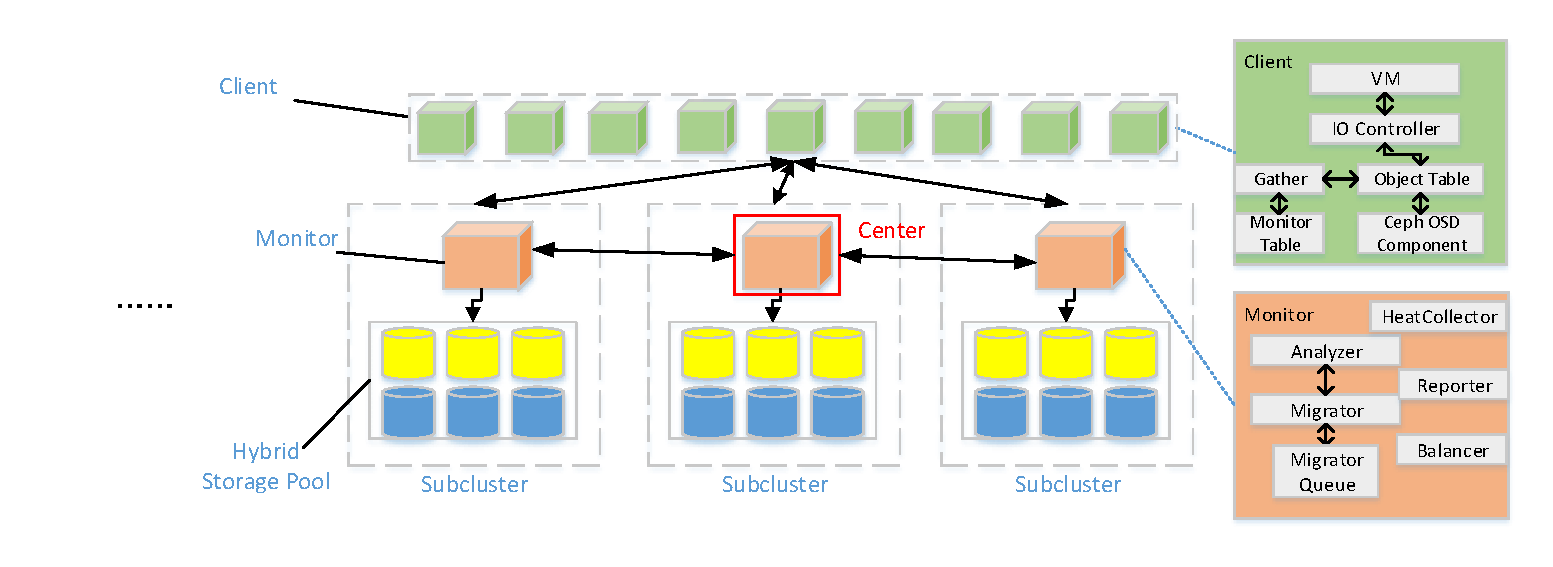
\includegraphics[width=16cm]{example/Arch.pdf}
    \bicaption[fig:arch]{DOBBS系统架构图}{DOBBS系统架构图}{Fig}{Architecture of DOBBS}
   \end{figure}

如图\ref{fig:arch}所示为DOBBS的系统架构图。DOBBS的架构大致可以分为两层,一层是存储集群也就是混合存储池,一层是监控器(Monitor)。DOBBS包含大量
的混合存储池以及监控器。存储集群正如上文所说的,它是有大量的混合存储池组成的。为了系统的高可靠性和高性能,我们将一个监控器和一个混合存储池绑定在一起,组成一个子
集群(subcluster)。之所以要划分成子集群是因为多个Monitor如果同时管理所有的混合存储池势必会造成管理的混乱,并大大降低系统的可扩展性。引入子集群则是可以充分
提升系统的可扩展性,并使整个系统易于管理。监控器在DOBBS则是起到至关重要的作用,它的作用包括监控虚拟机的数据流信息并生成合适的迁移策略,还有检测其所在子集群的热度并向中心节点(Center)
汇报,最终执行全局热均衡迁移指令。在DOBBS中,子集群仅仅只是逻辑上的概念,虚拟机VMDI则被均匀的分布在各个子集群的混合存储池中。监控器所监控的数据流信息也仅仅是其所在
子集群对应数据的数据流信息。客户端(Client)则是虚拟机管理器(VMM)所运行的机器,它们是DOBBS所提供服务的对象,客户端在接入DOBBS之后,与底层存储系统交互并进行数
据读写。中心节点则是DOBBS的监控器集群的大脑,它的主要作用是收集每个子集群的热度信息,并保证整个系统的热均衡。关于整个系统的热均衡,在本章后续章节将会叙述。

为了系统的高内聚低耦合,我们将系统分为多个模块,模块间互相依赖并支持高效扩展。在客户端上,如果让虚拟机管理器直接访问Ceph的块存储,那么它只需要调用Ceph提供的
OSD Component接口即可,但是为了获得虚拟机的数据流信息我们VM与Ceph存储设备的交互中间增加了一层DOBBS监控组件。因为Ceph是对象存储系统,所以虚拟机访问的粒度都是
一个个对象。如图\ref{fig:arch}所示,IO Controller负责截取VM的访问请求,然后通过查询Object Table来知道对象是在哪个OSD上,这是因为在数据迁移的过程中对象被频繁迁移,
而Ceph访问对象是通过对象ID和OSD共同组合访问,因此需要一个数据结构在存储对象ID和OSD ID的映射。Gather模块类似于一个计数器,它会记录每一个单位时间间隔内的
对象的访问次数、访问类型等信息,在记录之后再定时发送给Monitor。Monitor Table则是用来维护OSD ID和子集群ID映射的,因为在DOBBS在保证整个系统热均衡的过程中需要对OSD上的数据进行跨子集群迁移,所以
可能会导致某个OSD的位置发生了改变。最终,Ceph根据VM请求的对象ID和OSD ID来和底层存储进行交互。

Monitor主要有六个模块。Analyzer模块是Monitor的大脑,它负责接收客户端传送过来的虚拟机数据流信息,然后根据内置算法来生成合适的对象迁移命令,命令产生后将迁移命令传递给
Migrator模块执行。Migrator得到迁移指令之后,进行后续的上锁等等操作,然后再将最终的指令缓存在Migrator Queue中,这个队列的长度是DOBBS所支持的最大迁移数量,这个数量
当然也是可配置的。在Monitor上还有三个独立的模块,Reporter、HeatCollector和Blancer,他们都是用来负责系统热均衡的。

DOBBS提出了两个重要的概念,局部热均衡和全局热均衡。对于局部热均衡,我们数据对象分为两类,热对象和冷对象。所谓热对象是指的那些访问频率高,短时间内会被多次访问的对象。相反,
冷对象则是指那些访问频率并不高的对象。为了充分利用SSD的性能优势,我们将热对象都放置于SSD上而将冷对象都放置于HDD上,然后动态地监测数据对象的冷热变化来在SSD和HDD之间迁移对象。
局部热均衡只是针对每个子集群内部的局部热均衡,因此每个Monitor只能保证所在子集群的局部热均衡。

如果将存储集群和Monitor分割成多个子集群,那么极有可能在某个时刻某个虚拟机产生了非常大量的VMDI请求,这样某个子集群会遭受大量的读写请求,数据也会频繁地在SSD和HDD间迁移,这个子集群的效率将会受到极大
影响。提出全局热均衡的概念就是为了消除上述情况带来的性能波动。全局热均衡针对的粒度是OSD级别的,它会动态监测每个子集群的热度,然后做出迁移指令,有别于局部热均衡的迁移,全局热均衡的迁移是将OSD的数据进
行迁移而不是在OSD进行数据对象的迁移。

\section{局部热均衡}
因为SSD相较于HDD在读写速度上都有非常大的优势,并且SSD因为并不是采用机械的方式访问数据,所以也更加节能,在现在的数据中心中是存储的主流。但是,目前的SSD价格还是十分昂贵,容量
更是十分有限。如\citen{zhang2015skewly}所介绍的,冷数据和热数据实际也是符合80/20规律的,那么将数量较少的热数据放置于SSD数量较多的冷数据放置于HDD的策略是符合SSD容量小HDD容量大
特点的。DOBBS的局部热均衡则是动态地实现了数据的放置和迁移,我们从VM对数据的访问收集数据的信息,做出迁移策略。局部热均衡在保证存储效率的同时,也让整个存储的实现更加经济。值得注意的是局部
热均衡是针对每个子集群内部的热均衡。值得注意的的是,局部热均衡的基本设计思路是源自于WHOBBS\cite{lingxuan2015whobbs}的,而我们是在WHOBBS的基础上做出了修改和扩展。

\subsection{VM数据流监测和分析}
Ceph是一个对象存储系统,在VMDI创建之后,Ceph会把VMDI分割成大量对象存储于OSD上\cite{weil2006ceph}。因此局部热均衡锁面向的数据流信息指的是Ceph中每个对象的数据流信息。VM数据流的产生
源头是位于Client上的虚拟机管理器,如果安装原生Ceph的逻辑,虚拟机管理器直接和Ceph的OSD访问模块交互,进行数据读取。但是,我们需要获取VM数据流信息就必须将VM与Ceph的OSD访问模块截断。
当VM请求VMDI对象时,它会先经过IO Controller的访问控制。IO Controller主要实现两个功能,一是通过对象ID查询到OSD ID,二是记录这个对象的访问次数。之所以需要通过对象ID查询OSD ID,是因为
Ceph访问数据对象是通过对象ID和OSD ID共同组合访问的,但是局部热均衡会将对象在在OSD之间频繁移动,所以需要一个数据结构记录每个对象是在哪一个OSD上。Object Table就是用来记录对象位于哪个OSD
的数据结构。IO Controller通过对象ID在Object Table中查询VM请求对象所在的OSD,然后调用Ceph OSD Component来后续的对象读写。IO Controller的第二个功能是,记录这个请求对象的访问次数和
访问类型。在DOBBS中,我们刻画对象的数据流信息通过对象ID、访问类型(随机访问或顺序访问)以及单位时间内访问次数。IO Controller将截取的对象数据流信息交给Gather模块来进行统计和整合。Gather
模块在接收到IO Controller传递过来的数据流信息之后,记录下数据流信息,然后将单位时间内的数据流信息发送给Monitor,最后再清空计数器。

当Monitor收集到了从客户端节点发送来的数据流信息之后,它开始通过数据流信息计算每个对象的热度。这里提到的热度实际是一个具象化的数值。局部热均衡实际就是通过这个热值作为依据来进行对象的迁移。
Anlyzer模块就是主要负责,对象热值的计算以及得出合适的数据放置策略。考虑到虚拟机上运行的应用程序的多变性和复杂性,用一套通用的算法来计算数据对象的热度值并不是很现实。所以,DOBBS提供了更加
开放的方式,我们提供了算法接口API,这样用户可以直接继承这个接口来适配性地使用自己的热度值计算方法。我们还提供了一个默认的计算方法,沿用了WHOBBS\cite{lingxuan2015whobbs}的计算方法。

Anlyzer在计算完每个对象权重之后就开始启动周期性轮询机制产生对象迁移指令,它内部会维护一个有序的队列,这个队列描述了每一个对象热度值和其所在的OSD编号并且是通过每个对象的热度值降序排序。DOBBS做
SSD和HDD间的数据迁移是一种贪心的策略,我们始终保证热的对象可以占满整个SSD。所以,Anlyzer会周期性轮询有序队列,从对头取出一定数量的对象,让它们放置于SSD上。在系统刚刚加载时,我们默认所有对象
都位于HDD。Ceph默认的对象大小是64MB,所以根据SSD大小来决定多少个对象放置于SSD上。例如,128GB的SSD最多可以放置2000个对象,那么每次将队列头的2000个对象置于SSD,如果对象原来所在的位置是HDD,
则产生HDD到SSD的迁移指令。相反,如果遍历到对象是队列2000个以后,并且在SSD上的,则产生SSD到HDD的迁移指令。

\subsection{对象迁移}
Analyzer在产生迁移指令之后,Migrator则负责实际的对象迁移工作。Migrator首先会检查,当前的SSD是否已满,如果SSD已满则会终止掉当前的迁移请求。接下来,Migator将每一条迁移指令缓存下来,并存入迁移队列
Migrate Queue中。如果Migrator同时让多个对象进行迁移,那么对整个系统的性能将会是灾难性的影响。因为对象的传输将会大大占用网络带宽,并且DOBBS为了维护迁移过程中对象的一致性,需要频繁地对Client的对象
上锁和解锁,那么同时大量对象迁移将会影响VM的性能。所以,Migrate Queue保证了系统同时最大迁移数量,如果系统中已经有部分对象在做迁移,那么后续的迁移指令需要等待之前的迁移完成之后才可以执行。

DOBBS为了维护迁移过程中的一致性,会使用Remote Lock\cite{lingxuan2015whobbs}技术来对对象上锁,从而解决迁移过程中对一致性的破坏。试想这样一种情况,Analyzer所产生的迁移请求恰好是VM正在访问的对象,在DOBBS中对象迁移的优先级是很高的
,所以Client上的虚拟机可能在访问这个对象的时候丢失它,这样难免会造成数据的丢失,在一些数据关键型的应用中将带来难以估计的影响。Remote Lock就是做到了由Monitor向Client发起上锁请求,Client上锁成功后会向
Monitor发送上锁成功请求。只有Monitor在收到上锁成功请求后才会进行后续的迁移。

\section{全局热均衡}
\subsection{概念引入}
之所以要提出全局热均衡的概念要回到为什么将存储集群和Monitor集群划归成子集群的原因。在本章第二节介绍过,将集群分割为多个子集群是为了避免多Monitor共同管理存储集群可能带来的混乱。但是,分割成多个子集群之后
Client如何接入系统就会是一个问题,在DOBBS中我们对于全局热均衡有两个方面的考虑,一是静态的全局热均衡,二是动态的全局热均衡。

静态的全局热均衡就是Client在初次接入DOBBS系统时,Center会分配一个子集群给这个Client,Client在之后与系统的交互中就是和这个子集群的Monitor和底层存储之间进行。Center的分配规则
实际就是一种静态的负载均衡,Center会维护一个所有子集群热度的列表,它每次会把会“冷”的子集群分配给Client。通过这种方式,整个集群可以达到静态的负载均衡,但是随着每个VM上应用的不断变化,这种短暂的负载均衡终将打破。
所以,DOBBS在静态热均衡的基础上又加入了动态热均衡的设计。

假设这样一种情况,在一段时间内一个VM产生了极大量的VMDI请求并向某个子集群的Monitor汇报了大量的对象数据流信息,那么这样就会导致某一个子集群在突然承受非常大量的IO请求,而这个子集群的Monitor也需要处理大量的数据流
信息。就如上一节所说的,Monitor会保存一个有序队列,那么大量的数据信息将会导致Monitor频繁更新有序队列。这种情况会大大降低子集群上接入的其他Client的运行效率。为了解决这个问题,DOBBS采用动态热均衡的策略来动态监测每个
子集群的热度信息,然后做出决策找到最热的子集群再将热度扩散给其他子集群。

\subsection{热度不均衡监测}
热度不均衡出现在某个子集群在短时间内突然承受大量的VMDI请求,而如何刻画这一情况是全局热均衡关注的一个问题。我们观察发现子集群的热度主要有两个方面来刻画,一是存储集群的访问次数,二是Monitor的性能压力。因为Ceph的对象
大小是恒定的,所以只考虑存储集群的访问热度是合理的。Monitor上的Reporter模块是负责收集该子集群的热度信息。我们用单位时间内IO请求数来表示存储集群的热度,更加细致地来说,在DOBBS中我们用每秒IO(IO operations Per Second)来表示存
储集群的热度值。所以Reporter会调用内部接口实时监测存储集群所有OSD上的IOPS值,并进行汇总。而Monitor的热度我们用Monitor的CPU和内存利用率来表示,同样Reporter调用Linux系统调用来实时获取Monitor所在机器的CPU和内存利用率。
在获得了存储集群的IOPS和Monitor的使用率之后,Repoter将两者归一化之后组合起来,作为子集群的热度值。下面三个等式描述了子集群热度值的计算方式:


% \begin{equation}
%     \label{eq:stheat}
%     StorageHeat = \frac{\alpha \sum^n SIO + \beta \sum^m HIO}{m+n}
% \end{equation}

% \begin{equation}
%     \label{eq:monheat}
%     MonitorHeat = max(MemoryUsage, CPUUsage)
% \end{equation}

% \begin{equation}
%     \label{eq:subheat}
%     SubclusterHeat = StorageHeat + MonitorHeat
% \end{equation}

\begin{eqnarray}
    \displaystyle  StorageHeat = \frac{\alpha \sum^n SIO + \beta \sum^m HIO}{m+n} \label{eq:stheat}\\
    \displaystyle  MonitorHeat = max(MemoryUsage, CPUUsage) \label{eq:monheat}  \\
    \displaystyle  SubclusterHeat = StorageHeat + MonitorHeat
    \label{eq:subheat}
    \end{eqnarray}

等式\ref{eq:stheat}表示存储集群的热度,其中$SIO$和$HIO$分别表示SSD和HDD的IOPS值,$m$和$n$分别表示了子集群的存储集群内部SSD OSD的数量和HDD OSD的数量。$\alpha$和$\beta$是两个经验常数,在局部热均衡的过程中,我们已经将过热
的对象移动到SSD上而冷的对象放置于HDD上了,所以如果直接来看SSD和HDD对IOPS的贡献并不准确。$\alpha$和$\beta$起到了归一化的作用,他们是经过大量实验调参得到的数值。等式\ref{eq:monheat}表示的是Monitor的热度,这里的CPU利用率和
内存利用率都是用百分数表示的,之所以用二者的最大值是因为Monitor在处理大量数据流信息的时候需要存储在内存中,而计算是周期性的,所以用二者的最大值来表示Monitor的热度值。等式\ref{eq:subheat}则是将存储集群热度和Monitor热度相加来
表示子集群的热度值。Repoter定期计算所在子集群的热度信息,然后向Center节点汇报。

在Center节点上,它会保存所有子集群最新的热度值,在每次所有子集群汇报之后都会更新热度值。因此,Center节点总是保存最新的子集群的热度值。为了体现子集群热度的不均衡情况,我们用所有子集群热度的标准差来刻画子集群热度的不平衡,
那么标准差越大也就说明子集群的热度越不平衡。公式\ref{eq:sd}描述了子集群热度标准差的计算方法,其中$SubNum$表示子集群数量,$H_i$表示第i个子集群的热度值,而$\mu$则表示所有子集群热度值的均值。

\begin{equation}
    \label{eq:sd}
    heatSD = \sqrt{\frac{1}{SubNum} \sum_{i=0}^{SubNum} (H_i - \mu)^2}
\end{equation}

当然,仅仅根据子集群间的热度不均衡来触发全局热均衡必然是不充分的,我们还通过一个阈值来表示是否有子集群过热,如果出现一个子集群的热度值超过阈值,则会触发全局热均衡。我们通过下面的算法来判断
是否需要启动全局热均衡,并确定应该从哪个子集群开始做全局热均衡。因为集群的大小,接入系统的VM所运行的应用都不尽相同,所以我们让用户可以配置热度阈值和标准差阈值。

算法\ref{algo:imbadect}第1-3行是准备工作,获得热度值最大的子集群编号和热度值,计算实时集群热度值的标准差以及初始化当前热均衡迁移数量。第4-22行是算法的主循环,当存在一个
子集群热度值大于阈值或者当前标准差大于标准差阈值,则进入主循环进行后续的操作,否则终止算法。第5行保证了,整个系统的全局热均衡迁移的数量被控制在一个范围内,这样不会让大量热均衡迁移破坏整个
集群的效率,如果已经已经到达了最大数量,那么将重新获得标准差和最大热度值的子集群。第6行表示获取当前集群热度最低的子集群,我们将热度最低的子集群作为全局热均衡迁移的对象。第8-16行则表示了
如果集群中热度值最低的子集群的热度仍大于最大热度阈值,将等待出现比阈值小的子集群,否则在尝试一定次数之后就中断整个监控算法,然后想用户抛出异常,通知用户所有子集群的热度值都超过了阈值,提醒系
统管理员可能需要增加硬件。第13行的$sleep()$函数是因为所有子集群可能都存在过热的情况,我们等待一段时间后看是否有所缓解,第17行则表示,算法已经寻找到了源子集群和目标子集群,并启动全局热均
衡迁移,同时更新当前迁移数量。

可以看出算法\ref{algo:imbadect}的时间复杂度并不高,在实际情况中,Center会一直执行这个段算法,如果遇到算法退出或者终止,它将自动检测问题并重新启动检测算法。从算法可以看出,如果没有子集群的热度到达
阈值并且标准差没有达到阈值,将不启动检测程序,但是我们还是需要实时检测各个子集群的运行情况,在Center中还会启动一个线程来专门循环执行这个算法,直至算法异常退出。

\begin{algorithm}
    % \begin{algorithm}[H] % 强制定位
    \caption{子集群热度不均衡检测算法}
    \label{algo:imbadect}
    \begin{algorithmic}[1] %每行显示行号
    \Require $H_k$:子集群k的热度值,$HT$:用户自定义的热度阈值,$M$:最大热均衡迁移数量,$DT$:用户自定义的标准差阈值,$SubNum$:子集群数量
    \State {$H_i \gets getLargestHeatValue()$}
    \State {$currentSD \gets getCurrentStandardDeviation()$}
    \State {$currentMigration \gets 0 $}
    
    \While {$ H_i > HT$ or $currentSD > DT$}
      \If{$currentMigration < M$}
        \State {$H_j \gets getSmallestHeatValue()$}
        \State {$tryTimes \gets 0 $}
        \While{$H_j > HT$}
          \State $//$ All sub clusters are overheated
          \If{$ tryTimes > SubNum$}
            \State{$abortDetection()$}
          \EndIf
          \State {$sleep()$}
          \State {$H_j \gets getSmallestHeatValue()$}
          \State{$tryTimes \gets tryTimes + 1$}
        \EndWhile
        \State{ $applyMigration(i, j)$ }
        \State {$currentMigration \gets currentMigration + 1 $}
      \EndIf
      \State {$currentSD \gets getCurrentStandardDeviation()$}
      \State {$H_i \gets getLargestHeatValue()$}
    \EndWhile
    \end{algorithmic}
\end{algorithm}

如果我们用一个单独的节点(计算机)来作为Center,那么就必须保证这个Center节点的高可用性。因为如果DOBBS中的Center节点因为一些不可预料的因素宕机或是无法连通,那么对于整个系统来说将是致命的。Center
在整个集群中的作用是在Client接入系统是向Client分配较冷的一个子集群,还有就是收集每个子集群的热度值并做决策后发出热迁移指令。Center如果宕机或无法响应之后,那么新Client将无法接入系统,并且所有子集群可能
会处于一个热度极度不均衡的状态。不管是哪个问题,对DOBBS来说都是灾难性的。那么,如果用一个单独的计算机作为Center,它就变成了整个系统的唯一关键节点,一个合适的解决方法就是使用高效的一致性协议,让多个节点维护
该节点数据的大量备份,当这个节点宕机之后,根据一致性协议则可以快速切换Center。如此便保证了整个系统的高可用性。在DOBBS中,我们不再使用一个单独的节点作为Center,而是使用Raft\cite{ongaro2014search}这个
一致性协议,我们让集群中的某个Monitor作为Raft中的leader,同样也是Center,而其他Monitor用作备份节点,一旦这个leader宕机了,那么Raft将快速选举出一个Monitor作为Center。

本小结都是对全局热均衡的准备工作,包括如何定义子集群热度值和对子集群热度值的检测。

\subsection{热扩散}
上一小节介绍了DOBBS全局热均衡的前半部分的工作,本小节将介绍全局热均衡的全局热均衡迁移过程,这也是全局热均衡的重点。全局热均衡迁移过程在本论文中被称作热扩散过程,因为这个过程和物理上的热扩散十分相似,所以我们
就借用了热扩散的概念来概括全局热均衡迁移。物理上的热扩散过程指的是,理想情况下,热量会从热的物质向冷的物质扩散,最终两者的热量达到总量上一致。而在DOBBS上,我们指的是热量会从过热的子集群向一个相对热度值较低的
子集群扩散,最终两者的热度值达到总量上的一致。过热的子集群和热度较低的子集群都是由算法\ref{algo:imbadect}得到的,我们分别称它们为源子集群和目标子集群。

热扩散过程的目的是将源子集群过热的数据扩散到目标子集群上。与局部热均衡的迁移过程不同,局部热均衡是在子集群内部,多个OSD之间迁移数据对象,而热扩散过程则是跨子集群的迁移整个OSD的数据。DOBBS的策略是,源子集群在
接收到Center发送过来的迁移请求之后,它会去查询内部的HeatCollector,根据HeatCollector可以知道哪个OSD的IOPS最高,然后以这个OSD作为要迁移的OSD。然后目标子集群也会去查询自己HeatCollector,根据它的HeatCollector
就可以知道哪个OSD的IOPS最低,然后将这个OSD作为要被OSD。热扩散过程不能被认为是迁移的过程,它实际上是两个子集群交换OSD的过程。我们在介绍DOBBS系统架构的时候提到过,子集群只是一个逻辑上的概念,而每个子集群之间其实在
物理网络层面上是互联互通的,所以互相交换OSD是可行的,并且交换OSD只是在逻辑层面上交换,所以对整个集群的物理结构并没有任何影响。

但是大规模的数据传输对系统性能来说也是致命的。因为热扩散的过程是将整个OSD的数据进行交换,这样会带来两方面的性能上的影响。在下一章我们将介绍局部热均衡迁移的过程中,会出现因为数据对象的迁移导致上层虚拟机不能正确访问数据对象的问题,这
也是因为对象迁移带来的一致性问题,在系统实现的过程中我们使用了Remote Lock这一技术来解决这问题。Remote Lock会对Client上的数据对象上锁,在迁移过程中VM是不能访问到该对象的。那么,如果是将整个OSD迁移,一个OSD的大小大致是120G,而一个
Ceph对象的默认大小是64MB。如果将整个OSD迁移的话,因为Remote Lock的影响,迁移过程会导致Client上的对象被频发上锁、解锁,于是VM会被暂停运行。在局部热均衡中,一次只是对一个对象迁移,所以上锁带来的影响微乎其微,但是大量对象被上锁解锁,那么
对于VM是灾难性的。而如果VM上运行的实时应用程序,那更是难以想象的灾难。还有一个方面的性能问题,两个SSD的数据一共有240GB,那么传输过程也会非常久,而且占用大量集群核心网络的带宽。因此,如果将两个OSD的全部对象进行迁移则十分不现实,也严重
影响集群效率。

为了解决这个问题,我们采用了一个全新的懒汉迁移方式——元数据迁移。前面我们讲过直接将整个OSD的数据进行迁移是不现实的,那么这种方式可以定义成是一种饿汉迁移方式。借用物理学规律,我们知道热量的传递过程也是相对缓慢的,所以我们选择了一种慢速的迁移方式。
元数据迁移,是一种运用到DOBBS系统架构和局部热均衡的迁移方式,元数据指的是局部热均衡中的Analyzer所维护的数据流信息。在局部热均衡中,我们介绍过数据流信息包括每个对象的热度值以及它所在OSD的编号等信息。在源子集群收到Center的热扩散请求之后,它会先
检查HeatCollector,得到当前IOPS最大的OSD编号,之后再在Analyzer中再把属于这个最大IOPS OSD所有的对象数据流信息从有序队列中删除,并通过网络传输给目标子集群的Monitor。在目标子集群收到Center发送过来的热扩散请求之后,它会做相似的工作:目标子集群会先
检查HeatCollector,得到当前IOPS最小的OSD编号,之后再和源子集群的做法相同,然后再通过网络发送给目的子集群。因为DOBBS中,子集群是一个逻辑概念,所以每个子集群的Monitor都会本子集群所有OSD编号的列表。在源子集群和目标子集群互换原信息之后,它们也会修改所在
子集群的OSD信息。

\begin{figure}[!htp]
    \centering
    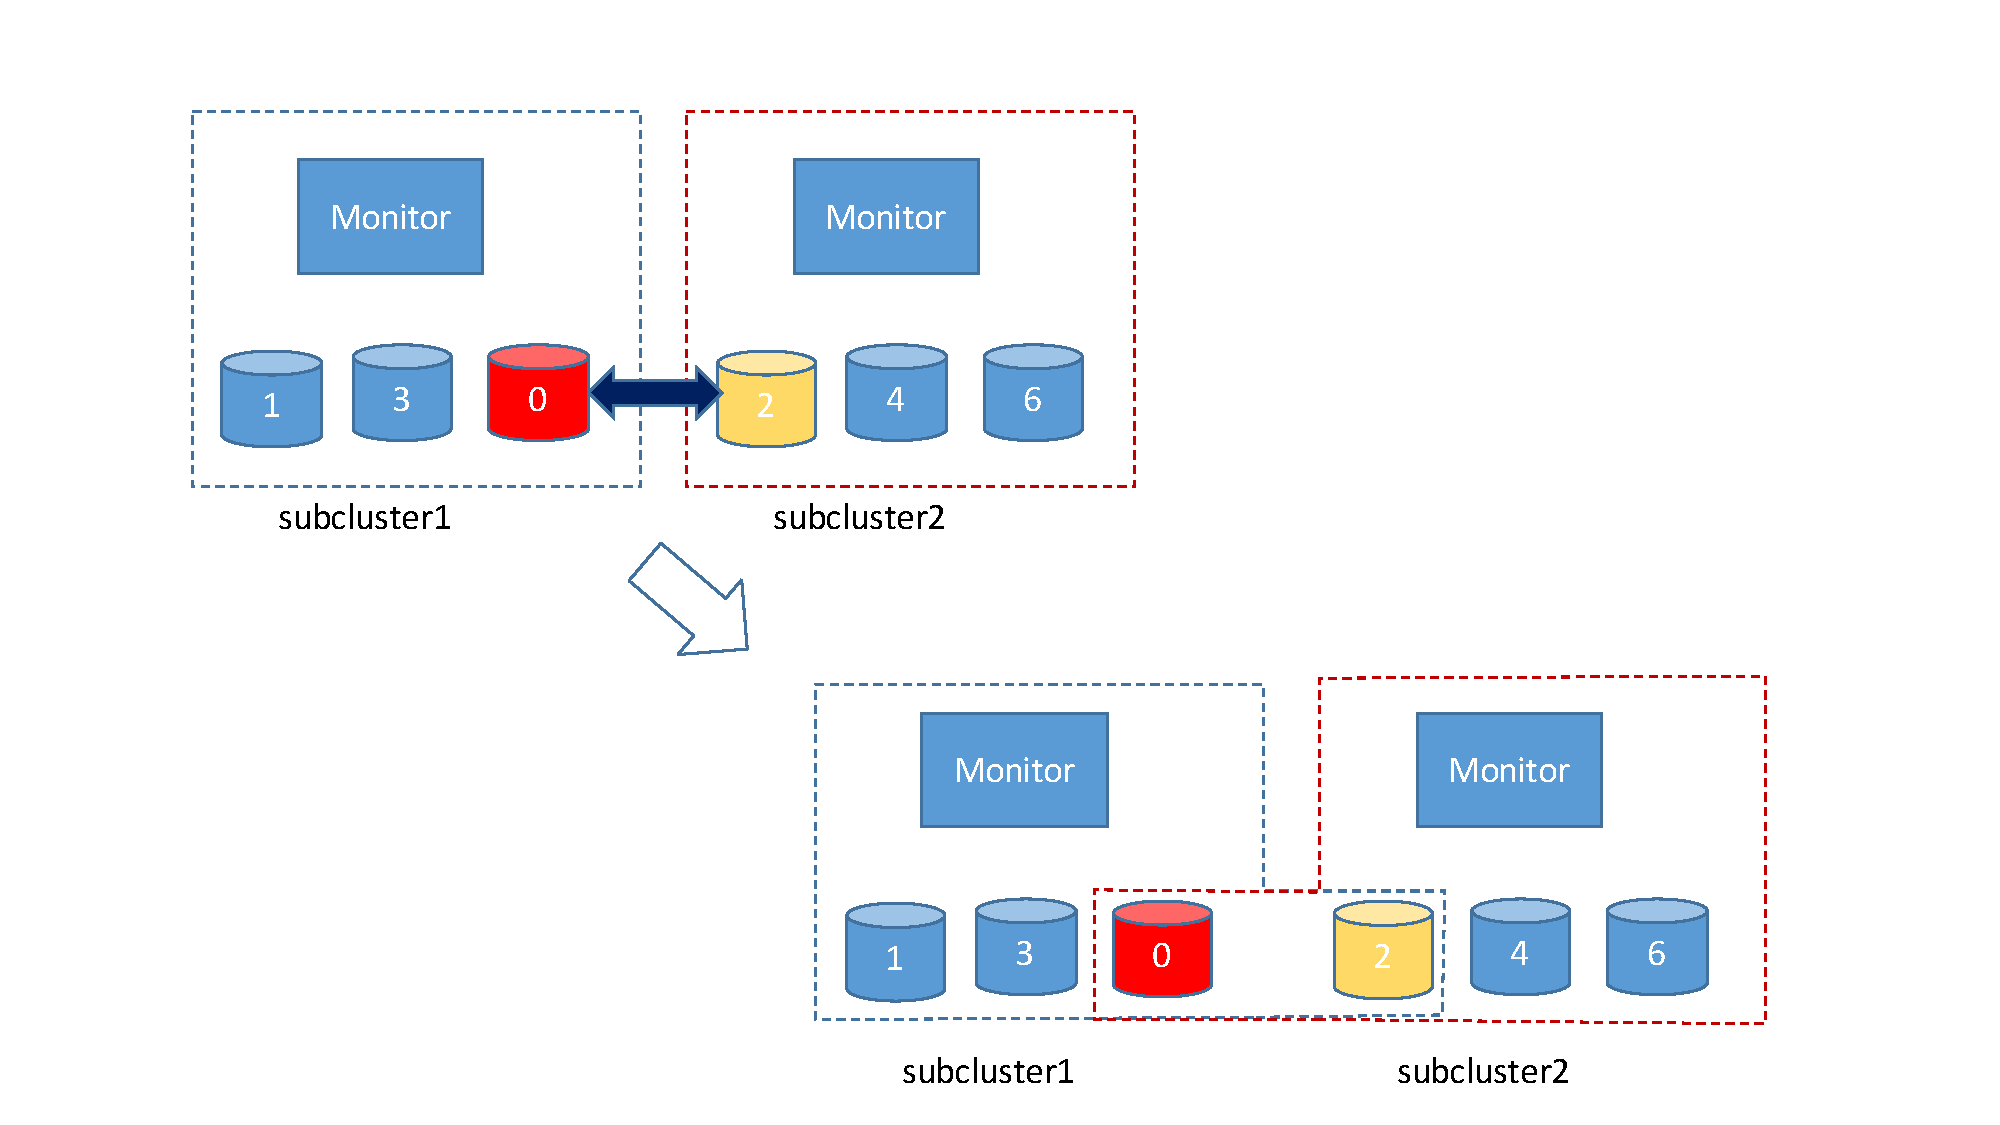
\includegraphics[width=15cm]{example/heatdiffusion0.pdf}
    \bicaption[fig:heatdiffison0]{元数据迁移使能过程}{元数据迁移使能过程}{Fig}{Enable Process of Metadata Migration}
\end{figure}

元数据迁移的过程是可以证明有效的。元数据迁移和饿汉模式相比,并没有做物理上的数据迁移,而仅仅从逻辑上改变了两个存储集群的中OSD的位置。例如,原来子集群1包含第0、1、3号OSD,而子集群2包含第2、4、6号OSD,现在子集群1作为源子集群,子集群2作为目标子集群,它们交换了
第0和第2号OSD,那么现在子集群1就包含第2、1、3号OSD,而子集群2包含了第0、4、6号OSD。图\ref{fig:heatdiffison0}所示,就是上面所举的例子的示意图。可以从图中看出元数据迁移只是修改了OSD的逻辑结构,而并没有在两个OSD上互相交换数据。在最终交换完成后,只是完成了
元数据迁移的使能过程。

我们将元数据迁移分为两个过程,一个是使能过程,还有一个是懒迁移过程。使能过程也就上上文所提到的,两个子集群修改自身的逻辑结构,然后两个Monitor交换元数据的过程。当然从使能过程的结果来看,其实并没有真正的实现热量的转移,而只是修改了逻辑结构,对问题的本质并没有实质性的
影响。我们成元数据迁移是一种混合的方式,懒迁移过程实际有局部热均衡参与。我们将源子集群的属于IOPS最大OSD的元数据拷贝到了目标子集群的Anlyzer中,从目标子集群的Analyzer角度看来,就像是从Client新汇报出大量数据对象。根据上一节我们寻找源子集群和目标子集群的策略可以知道,
目标子集群一定是当前热度值最低的子集群,而源子集群一定是当前热度值最高的子集群,并且我们所交换的OSD也是它们彼此最“冷”和最“热”的OSD。所以,目标子集群所收到的元数据的热度值一定是比其自身所有OSD上对象的热度值的最大值都要大的。根据局部热均衡的原理,目标子集群Analyzer在
收到这些热度值很高的元数据之后,它会优先将这些元数据所对应的数据对象迁移到它的SSD OSD上。相反,在源子集群接收到目标子集群的元数据之后,它会优先将这些元数据锁对应的对象进行转移。当然,具体是如何转移要依照具体情况决定。这个过程就是,元数据迁移的懒迁移过程,可以看到我们
并没有让Monitor立即去迁移所有的数据,而是交给了局部热均衡去做迁移的工作,这相当于是一种缓慢的迁移方式。元数据迁移是有效的,因为在修改OSD的逻辑结构之后,局部热均衡充当了迁移者,它把过热的OSD上的热量辐射到目标子集群的其他OSD上去,做到了热量扩散。

元数据迁移过程的使能过程的迁移对象是对象的数据流信息(元数据),这个数据流信息实际上是局部热均衡用来决策的重要依据。假设有这样一个情况,在局部热均衡的过程中,某个Monitor正在执行对象迁移指令,它向Client发送了上锁指令,随即Client对要被迁移的对象上锁,可是在这次对象
迁移过程没有执行完之前,该Monitor又收到了元数据迁移请求,它立即响应请求将部分元数据传送到目标子集群。在元数据迁移完成后,OSD已经互相交换,并且Client上的Monitor Table也已经被更新。那么,Monitor则始终不能发送release-lock请求对应的Client,Client上的这个对象可能
会被永久得阻塞,这样Client上运行的VM也将受到影响。为了解决这个问题,我们提出了一个try-lock机制。该机制会首先尝试从源子集群和目标子集群上获得锁,但是如果其中有子集群正在执行局部热均衡的对象迁移,则返回失败,即不能获得锁。当且仅当Center获得了源子集群和目标子集群的两个锁
之后才算上锁成功,才可以继续元数据迁移。在两个集群上的锁,一旦上锁之后,Monitor就不能产生对象迁移请求,直到锁释放才可以进行对象迁移。

\begin{figure}[!htp]
    \centering
    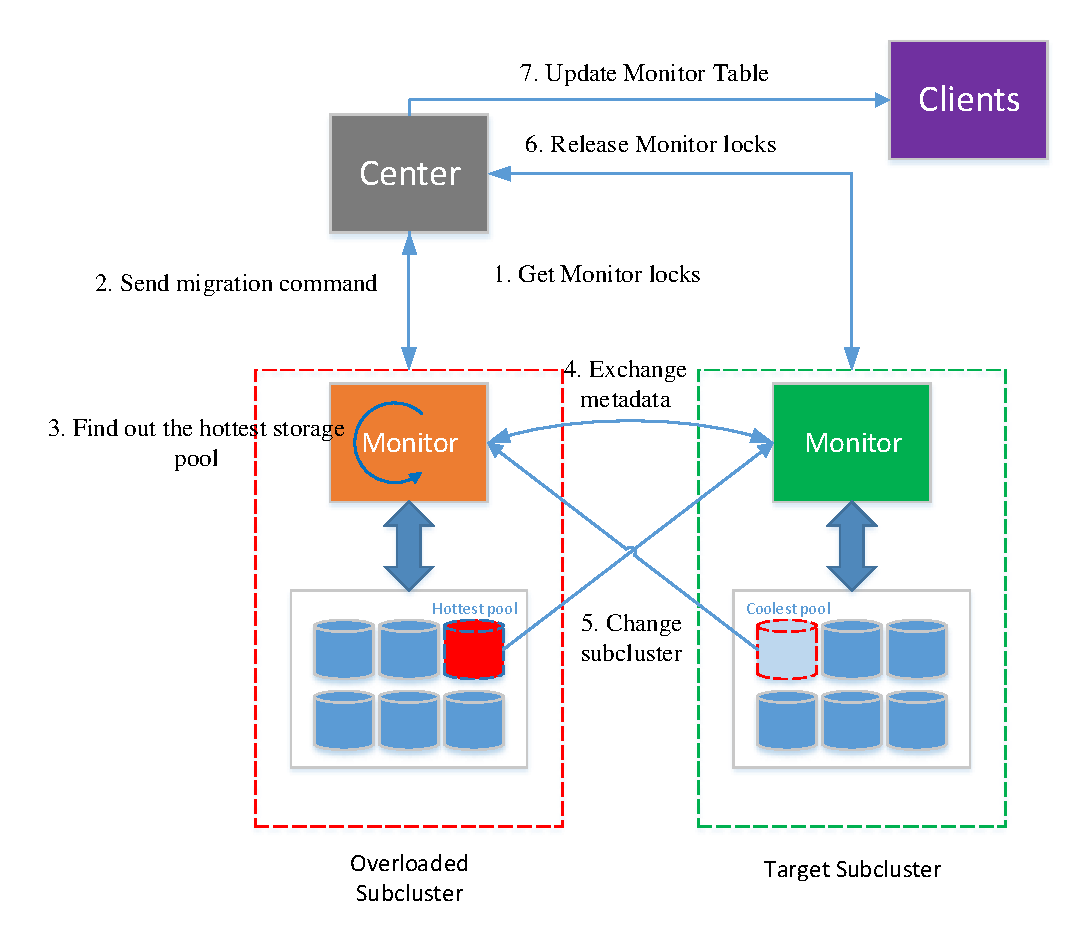
\includegraphics[width=12cm]{example/MetaDataMigration.pdf}
    \bicaption[fig:heatdiffison1]{热扩散过程}{热扩散过程}{Fig}{Process of Heat Diffusion}
\end{figure}

图\ref{fig:heatdiffison1}所示为DOBBS的热扩散过程的示意图。热扩散过程可以总结成7个步骤,在Center找到需要被扩散的源子集群和目标子集群之后,它会首先通过try-lock机制向两个子集群的Monitor获得锁。只有当同时过得两把锁之后,Center执行第二步也就是向源子集群和目标子集群发送
元数据迁移指令。两个子集群的Monitor接受到指令之后,它们查询各自的HeatCollector,然后将元数据进行交换,再修改两个子集群的存储逻辑结构,两个Monitor更新各自的OSD列表。在这些过程结束之后,Center释放两个子集群的锁,并更新Client上的Monitor Table。一旦锁被释放,两个Monitor
就开始进行局部热均衡,也就是开始懒迁移过程。

\section{本章小结}
本章主要从DOBBS系统的架构、局部热均衡、全局热均衡等三个方面介绍了系统的设计。DOBBS的架构是采用了一种两层的架构方式,整个系统主要有4中类型的节点,其中Client节点是搭载虚拟机的节点,Monitor是每个子集群的监视器,Center则负责全局热均衡,最后就是OSD节点。OSD根据存储介质被分成了
SSD OSD和HDD OSD。DOBBS还将Monitor和混合存储池合并成一个逻辑结构——子集群。局部热均衡是为了充分利用SSD的优势,并以一个经济的方式实现混合存储,我们通过动态监测对象的数据流信息计算对象热度来迁移对象到合适的OSD上。全局热均衡则是因为我们采用分布式多节点Monitor之后产生的数据访问
不均衡现象,所以要通过一种动态的方式来进行负载均衡,也就是热量的传递。

